% 2020 May 18 - THE MARTIAN ATMOSPHERIC BOUNDARY LAYER - https://agupubs.onlinelibrary.wiley.com/doi/10.1029/2010RG000351


%% Beginning of file 'sample63.tex'
%%
%% Modified 2019 June
%%
%% This is a sample manuscript marked up using the
%% AASTeX v6.3 LaTeX 2e macros.
%%
%% AASTeX is now based on Alexey Vikhlinin's emulateapj.cls 
%% (Copyright 2000-2015).  See the classfile for details.

%% AASTeX requires revtex4-1.cls (http://publish.aps.org/revtex4/) and
%% other external packages (latexsym, graphicx, amssymb, longtable, and epsf).
%% All of these external packages should already be present in the modern TeX 
%% distributions.  If not they can also be obtained at www.ctan.org.

%% The first piece of markup in an AASTeX v6.x document is the \documentclass
%% command. LaTeX will ignore any data that comes before this command. The 
%% documentclass can take an optional argument to modify the output style.
%% The command below calls the preprint style which will produce a tightly 
%% typeset, one-column, single-spaced document.  It is the default and thus
%% does not need to be explicitly stated.
%%
%%
%% using aastex version 6.3
\usepackage{amsmath}
\documentclass{aastex63}

%% The default is a single spaced, 10 point font, single spaced article.
%% There are 5 other style options available via an optional argument. They
%% can be invoked like this:
%%
%% \documentclass[arguments]{aastex63}
%% 
%% where the layout options are:
%%
%%  twocolumn   : two text columns, 10 point font, single spaced article.
%%                This is the most compact and represent the final published
%%                derived PDF copy of the accepted manuscript from the publisher
%%  manuscript  : one text column, 12 point font, double spaced article.
%%  preprint    : one text column, 12 point font, single spaced article.  
%%  preprint2   : two text columns, 12 point font, single spaced article.
%%  modern      : a stylish, single text column, 12 point font, article with
%% 		  wider left and right margins. This uses the Daniel
%% 		  Foreman-Mackey and David Hogg design.
%%  RNAAS       : Preferred style for Research Notes which are by design 
%%                lacking an abstract and brief. DO NOT use \begin{abstract}
%%                and \end{abstract} with this style.
%%
%% Note that you can submit to the AAS Journals in any of these 6 styles.
%%
%% There are other optional arguments one can invoke to allow other stylistic
%% actions. The available options are:
%%
%%   astrosymb    : Loads Astrosymb font and define \astrocommands. 
%%   tighten      : Makes baselineskip slightly smaller, only works with 
%%                  the twocolumn substyle.
%%   times        : uses times font instead of the default
%%   linenumbers  : turn on lineno package.
%%   trackchanges : required to see the revision mark up and print its output
%%   longauthor   : Do not use the more compressed footnote style (default) for 
%%                  the author/collaboration/affiliations. Instead print all
%%                  affiliation information after each name. Creates a much 
%%                  longer author list but may be desirable for short 
%%                  author papers.
%% twocolappendix : make 2 column appendix.
%%   anonymous    : Do not show the authors, affiliations and acknowledgments 
%%                  for dual anonymous review.
%%
%% these can be used in any combination, e.g.
%%
%% \documentclass[twocolumn,linenumbers,trackchanges]{aastex63}
%%
%% AASTeX v6.* now includes \hyperref support. While we have built in specific
%% defaults into the classfile you can manually override them with the
%% \hypersetup command. For example,
%%
%% \hypersetup{linkcolor=red,citecolor=green,filecolor=cyan,urlcolor=magenta}
%%
%% will change the color of the internal links to red, the links to the
%% bibliography to green, the file links to cyan, and the external links to
%% magenta. Additional information on \hyperref options can be found here:
%% https://www.tug.org/applications/hyperref/manual.html#x1-40003
%%
%% Note that in v6.3 "bookmarks" has been changed to "true" in hyperref
%% to improve the accessibility of the compiled pdf file.
%%
%% If you want to create your own macros, you can do so
%% using \newcommand. Your macros should appear before
%% the \begin{document} command.
%%
\newcommand{\vdag}{(v)^\dagger}
\newcommand\aastex{AAS\TeX}
\newcommand\latex{La\TeX}

%% Reintroduced the \received and \accepted commands from AASTeX v5.2
\received{June 1, 2019}
\revised{January 10, 2019}
\accepted{\today}
%% Command to document which AAS Journal the manuscript was submitted to.
%% Adds "Submitted to " the argument.
\submitjournal{PSJ}

%% For manuscript that include authors in collaborations, AASTeX v6.3
%% builds on the \collaboration command to allow greater freedom to 
%% keep the traditional author+affiliation information but only show
%% subsets. The \collaboration command now must appear AFTER the group
%% of authors in the collaboration and it takes TWO arguments. The last
%% is still the collaboration identifier. The text given in this
%% argument is what will be shown in the manuscript. The first argument
%% is the number of author above the \collaboration command to show with
%% the collaboration text. If there are authors that are not part of any
%% collaboration the \nocollaboration command is used. This command takes
%% one argument which is also the number of authors above to show. A
%% dashed line is shown to indicate no collaboration. This example manuscript
%% shows how these commands work to display specific set of authors 
%% on the front page.
%%
%% For manuscript without any need to use \collaboration the 
%% \AuthorCollaborationLimit command from v6.2 can still be used to 
%% show a subset of authors.
%
%\AuthorCollaborationLimit=2
%
%% will only show Schwarz & Muench on the front page of the manuscript
%% (assuming the \collaboration and \nocollaboration commands are
%% commented out).
%%
%% Note that all of the author will be shown in the published article.
%% This feature is meant to be used prior to acceptance to make the
%% front end of a long author article more manageable. Please do not use
%% this functionality for manuscripts with less than 20 authors. Conversely,
%% please do use this when the number of authors exceeds 40.
%%
%% Use \allauthors at the manuscript end to show the full author list.
%% This command should only be used with \AuthorCollaborationLimit is used.

%% The following command can be used to set the latex table counters.  It
%% is needed in this document because it uses a mix of latex tabular and
%% AASTeX deluxetables.  In general it should not be needed.
%\setcounter{table}{1}

%%%%%%%%%%%%%%%%%%%%%%%%%%%%%%%%%%%%%%%%%%%%%%%%%%%%%%%%%%%%%%%%%%%%%%%%%%%%%%%%
%%
%% The following section outlines numerous optional output that
%% can be displayed in the front matter or as running meta-data.
%%
%% If you wish, you may supply running head information, although
%% this information may be modified by the editorial offices.
\shorttitle{Optimizing Imaging Surveys for Dust Devils}
\shortauthors{Jackson}
%%
%% You can add a light gray and diagonal water-mark to the first page 
%% with this command:
%% \watermark{text}
%% where "text", e.g. DRAFT, is the text to appear.  If the text is 
%% long you can control the water-mark size with:
%% \setwatermarkfontsize{dimension}
%% where dimension is any recognized LaTeX dimension, e.g. pt, in, etc.
%%
%%%%%%%%%%%%%%%%%%%%%%%%%%%%%%%%%%%%%%%%%%%%%%%%%%%%%%%%%%%%%%%%%%%%%%%%%%%%%%%%
\graphicspath{{./}{figures/}}
%% This is the end of the preamble.  Indicate the beginning of the
%% manuscript itself with \begin{document}.

\begin{document}

\title{Optimizing Imaging Surveys for Dust Devils}

%% LaTeX will automatically break titles if they run longer than
%% one line. However, you may use \\ to force a line break if
%% you desire. In v6.3 you can include a footnote in the title.

%% A significant change from earlier AASTEX versions is in the structure for 
%% calling author and affiliations. The change was necessary to implement 
%% auto-indexing of affiliations which prior was a manual process that could 
%% easily be tedious in large author manuscripts.
%%
%% The \author command is the same as before except it now takes an optional
%% argument which is the 16 digit ORCID. The syntax is:
%% \author[xxxx-xxxx-xxxx-xxxx]{Author Name}
%%
%% This will hyperlink the author name to the author's ORCID page. Note that
%% during compilation, LaTeX will do some limited checking of the format of
%% the ID to make sure it is valid. If the "orcid-ID.png" image file is 
%% present or in the LaTeX pathway, the OrcID icon will appear next to
%% the authors name.
%%
%% Use \affiliation for affiliation information. The old \affil is now aliased
%% to \affiliation. AASTeX v6.3 will automatically index these in the header.
%% When a duplicate is found its index will be the same as its previous entry.
%%
%% Note that \altaffilmark and \altaffiltext have been removed and thus 
%% can not be used to document secondary affiliations. If they are used latex
%% will issue a specific error message and quit. Please use multiple 
%% \affiliation calls for to document more than one affiliation.
%%
%% The new \altaffiliation can be used to indicate some secondary information
%% such as fellowships. This command produces a non-numeric footnote that is
%% set away from the numeric \affiliation footnotes.  NOTE that if an
%% \altaffiliation command is used it must come BEFORE the \affiliation call,
%% right after the \author command, in order to place the footnotes in
%% the proper location.
%%
%% Use \email to set provide email addresses. Each \email will appear on its
%% own line so you can put multiple email address in one \email call. A new
%% \correspondingauthor command is available in V6.3 to identify the
%% corresponding author of the manuscript. It is the author's responsibility
%% to make sure this name is also in the author list.
%%
%% While authors can be grouped inside the same \author and \affiliation
%% commands it is better to have a single author for each. This allows for
%% one to exploit all the new benefits and should make book-keeping easier.
%%
%% If done correctly the peer review system will be able to
%% automatically put the author and affiliation information from the manuscript
%% and save the corresponding author the trouble of entering it by hand.

\correspondingauthor{Brian Jackson}
\email{bjackson@boisestate.edu}

\author[0000-0002-9495-9700]{Brian Jackson}
\affiliation{Department of Physics\\ 
Boise State University\\ 
1910 University Drive, Boise ID 83725-1570 USA}

%% Note that the \and command from previous versions of AASTeX is now
%% depreciated in this version as it is no longer necessary. AASTeX 
%% automatically takes care of all commas and "and"s between authors names.

%% AASTeX 6.3 has the new \collaboration and \nocollaboration commands to
%% provide the collaboration status of a group of authors. These commands 
%% can be used either before or after the list of corresponding authors. The
%% argument for \collaboration is the collaboration identifier. Authors are
%% encouraged to surround collaboration identifiers with ()s. The 
%% \nocollaboration command takes no argument and exists to indicate that
%% the nearby authors are not part of surrounding collaborations.

%% Mark off the abstract in the ``abstract'' environment. 
\begin{abstract}


\end{abstract}

%% Keywords should appear after the \end{abstract} command. 
%% See the online documentation for the full list of available subject
%% keywords and the rules for their use.
\keywords{editorials, notices --- 
miscellaneous --- catalogs --- surveys}

%% From the front matter, we move on to the body of the paper.
%% Sections are demarcated by \section and \subsection, respectively.
%% Observe the use of the LaTeX \label
%% command after the \subsection to give a symbolic KEY to the
%% subsection for cross-referencing in a \ref command.
%% You can use LaTeX's \ref and \label commands to keep track of
%% cross-references to sections, equations, tables, and figures.
%% That way, if you change the order of any elements, LaTeX will
%% automatically renumber them.
%%
%% We recommend that authors also use the natbib \citep
%% and \citet commands to identify citations.  The citations are
%% tied to the reference list via symbolic KEYs. The KEY corresponds
%% to the KEY in the \bibitem in the reference list below. 

\section{Introduction} \label{sec:Introduction}

% 2020 May 16 - Discuss how Greeley et al. (2006) spotted and analyzed dust devils.

% \citet{2010Icar..206..306N} report a dust flux $Q$ that depends on the pressure deficit at the center of a vortex $\Delta P$ as
% \begin{equation}
%     Q = \left(5.79\times10^{-8} {\rm kg\ m^{-2}\ s^{-1}} \right) \left( \Delta P/{\rm Pa}\right)^{3.40}.
%     \label{eqn:Neakrase_dust_flux}
% \end{equation}
% \begin{figure}
%     \centering
%     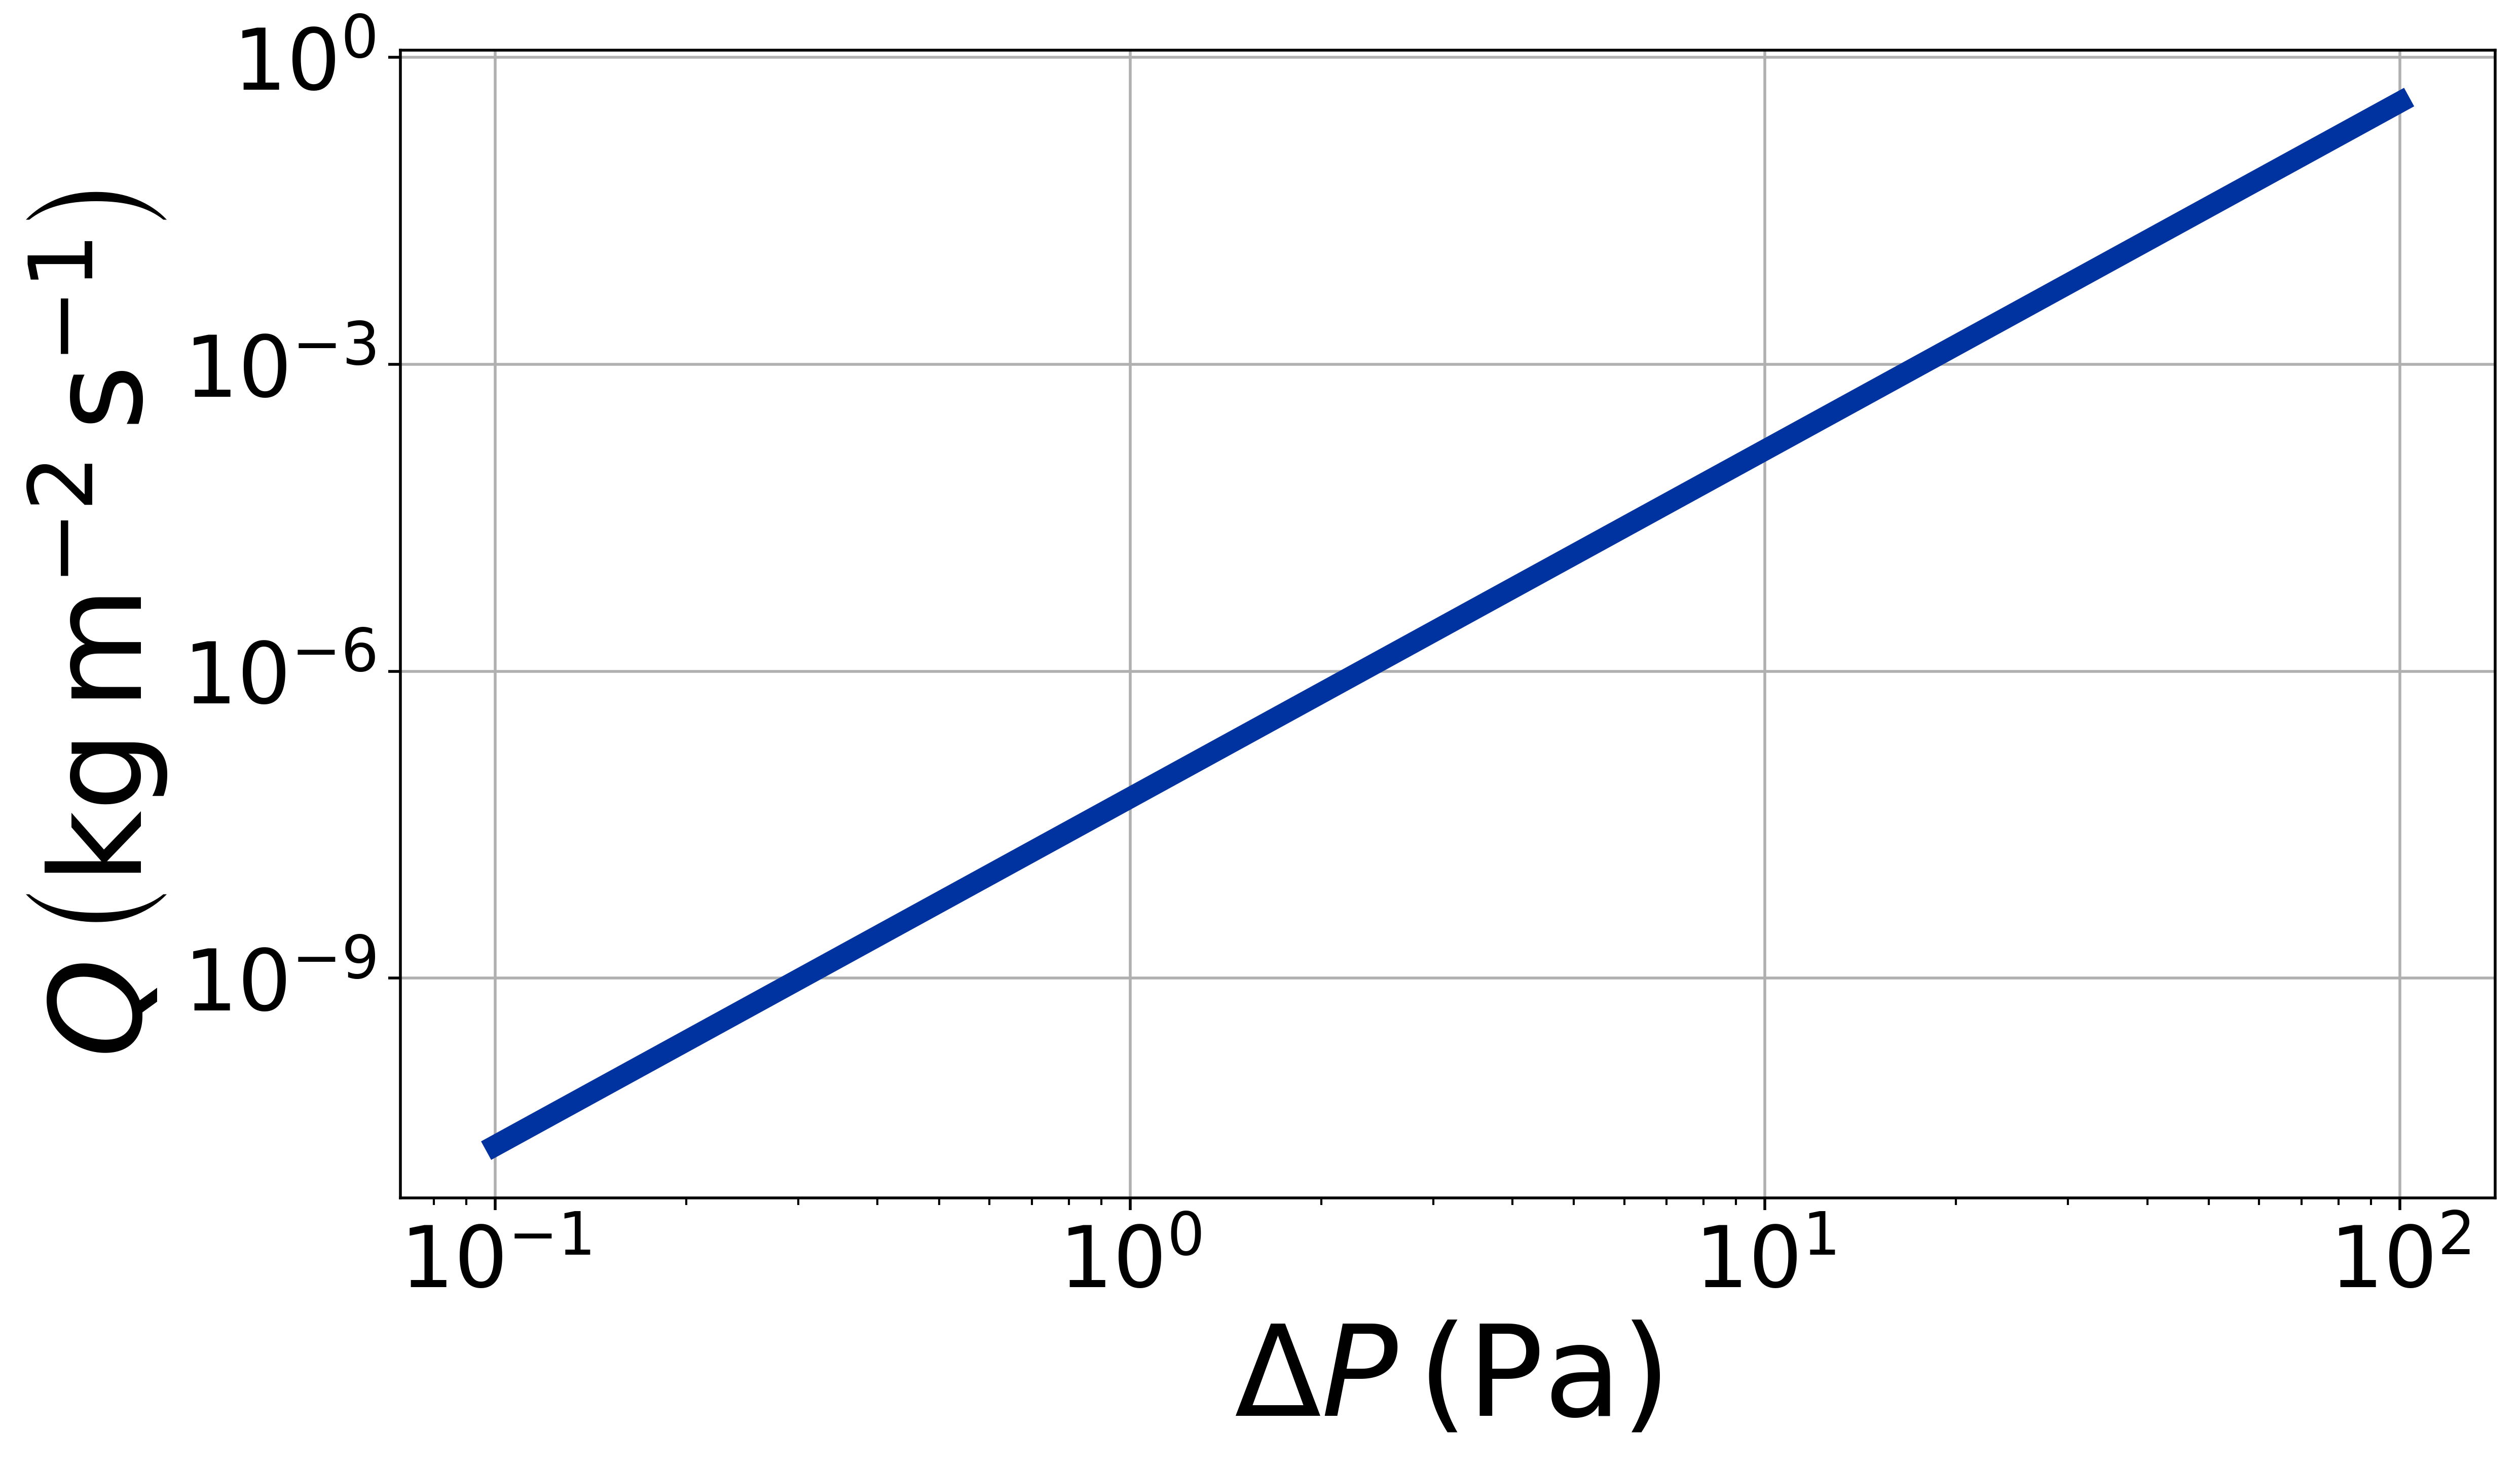
\includegraphics[width=\textwidth]{figures/Q_vs_Delta-P.png}
%     \caption{Dust flux $Q$ as a function of the pressure dip at the center of a lab-generated vortex $\Delta P$, as reported in \citet{2010Icar..206..306N}.}
%     \label{fig:Neakrase_dust_flux}
% \end{figure}

\section{Camera Model}

\begin{figure}
    \centering
    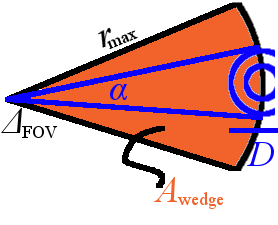
\includegraphics[width=0.5\textwidth]{figures/Awedge.jpg}
    \caption{Observational geometry. The camera has a field-of-view is $\Delta_{\rm FOV}$ and an angular resolution $\alpha$ which allows it to resolve dust devils of diameter $D$ out to a radial distance $r_{\rm max}$. The area surveyed is $A_{\rm wedge}$.}
    \label{fig:Awedge}
\end{figure}

Consider a camera with a horizontal field-of-view $\Delta_{\rm FOV}$ centered on azimuth $\lambda$ and an angular resolution $\alpha$ (Figure \ref{fig:Awedge}). Initially, we will assume the camera observes continuously throughout the period during which dust devils are active. Consider also a dust devil with a fixed diameter $D$, height $H$, and a sufficient contrast against the image background that it can be detected. Such a dust devil could be resolved at a distance from the camera $r_{\rm max} = \dfrac{D}{\alpha}$. 

In principle, the camera could detect this dust devil if it traversed the pie-wedge of terrain centered on $\lambda$ and having an area 
\begin{equation}
    A_{\rm wedge} = \frac{\Delta_{\rm FOV} r_{\rm max}^2}{2} = \frac{\Delta_{\rm FOV}D^2}{2 \alpha^2}.
    \label{eqn:A_wedge}
\end{equation}
Typical values for these parameters are $\Delta_{\rm FOV} \sim \pi/2\,{\rm rad}$, $D \sim 10\,{\rm m}$, and $\alpha \sim 1\,{\rm mrad}$, giving $A_{\rm wedge} \sim 100\,{\rm km^2}$ (although we will explore different values for these parameters). If dust devils traveled very slowly (or not at all) from their origin point, then the survey would only include devils that appeared within this wedge. However, as pointed out in \citet{2014JAtS...71.4461L}, advection of dust devils through a survey site increases the effective area surveyed. 

Consider a fixed, unidirectional wind of speed $U$ crossing perpendicularly through the pie-wedge. If the dust devil under consideration has a lifetime $\tau$, then it will travel a distance $L = \tau U$ before dissipating. Thus, the wind field can advect dust devils into the camera's field-of-view acting as a rectangular conveyor belt with area
\begin{equation}
    A_{\rm adv} = r_{\rm max} L = \frac{D U \tau}{\alpha}.
    \label{eqn:A_adv}
\end{equation}
Again, typical values $D \sim 10\,{\rm m}$, $U \sim 10\,{\rm m\ s^{-1}}$, $\tau \sim 100\,{\rm s}$, and $\alpha \sim 1\,{\rm mrad}$ gives $A_{\rm adv} \sim 10\,{\rm km^2} \ll A_{\rm wedge}$. Although both areas contribute, we neglect $A_{\rm adv}$ compared to $A_{\rm wedge}$, and we use this estimate for the area surveyed $A_{\rm survey} \approx A_{\rm wedge}$ to determine how the inferred population of dust devils depends on the survey parameters.

\section{Imaging Survey Statistics}

\begin{figure}
    \centering
    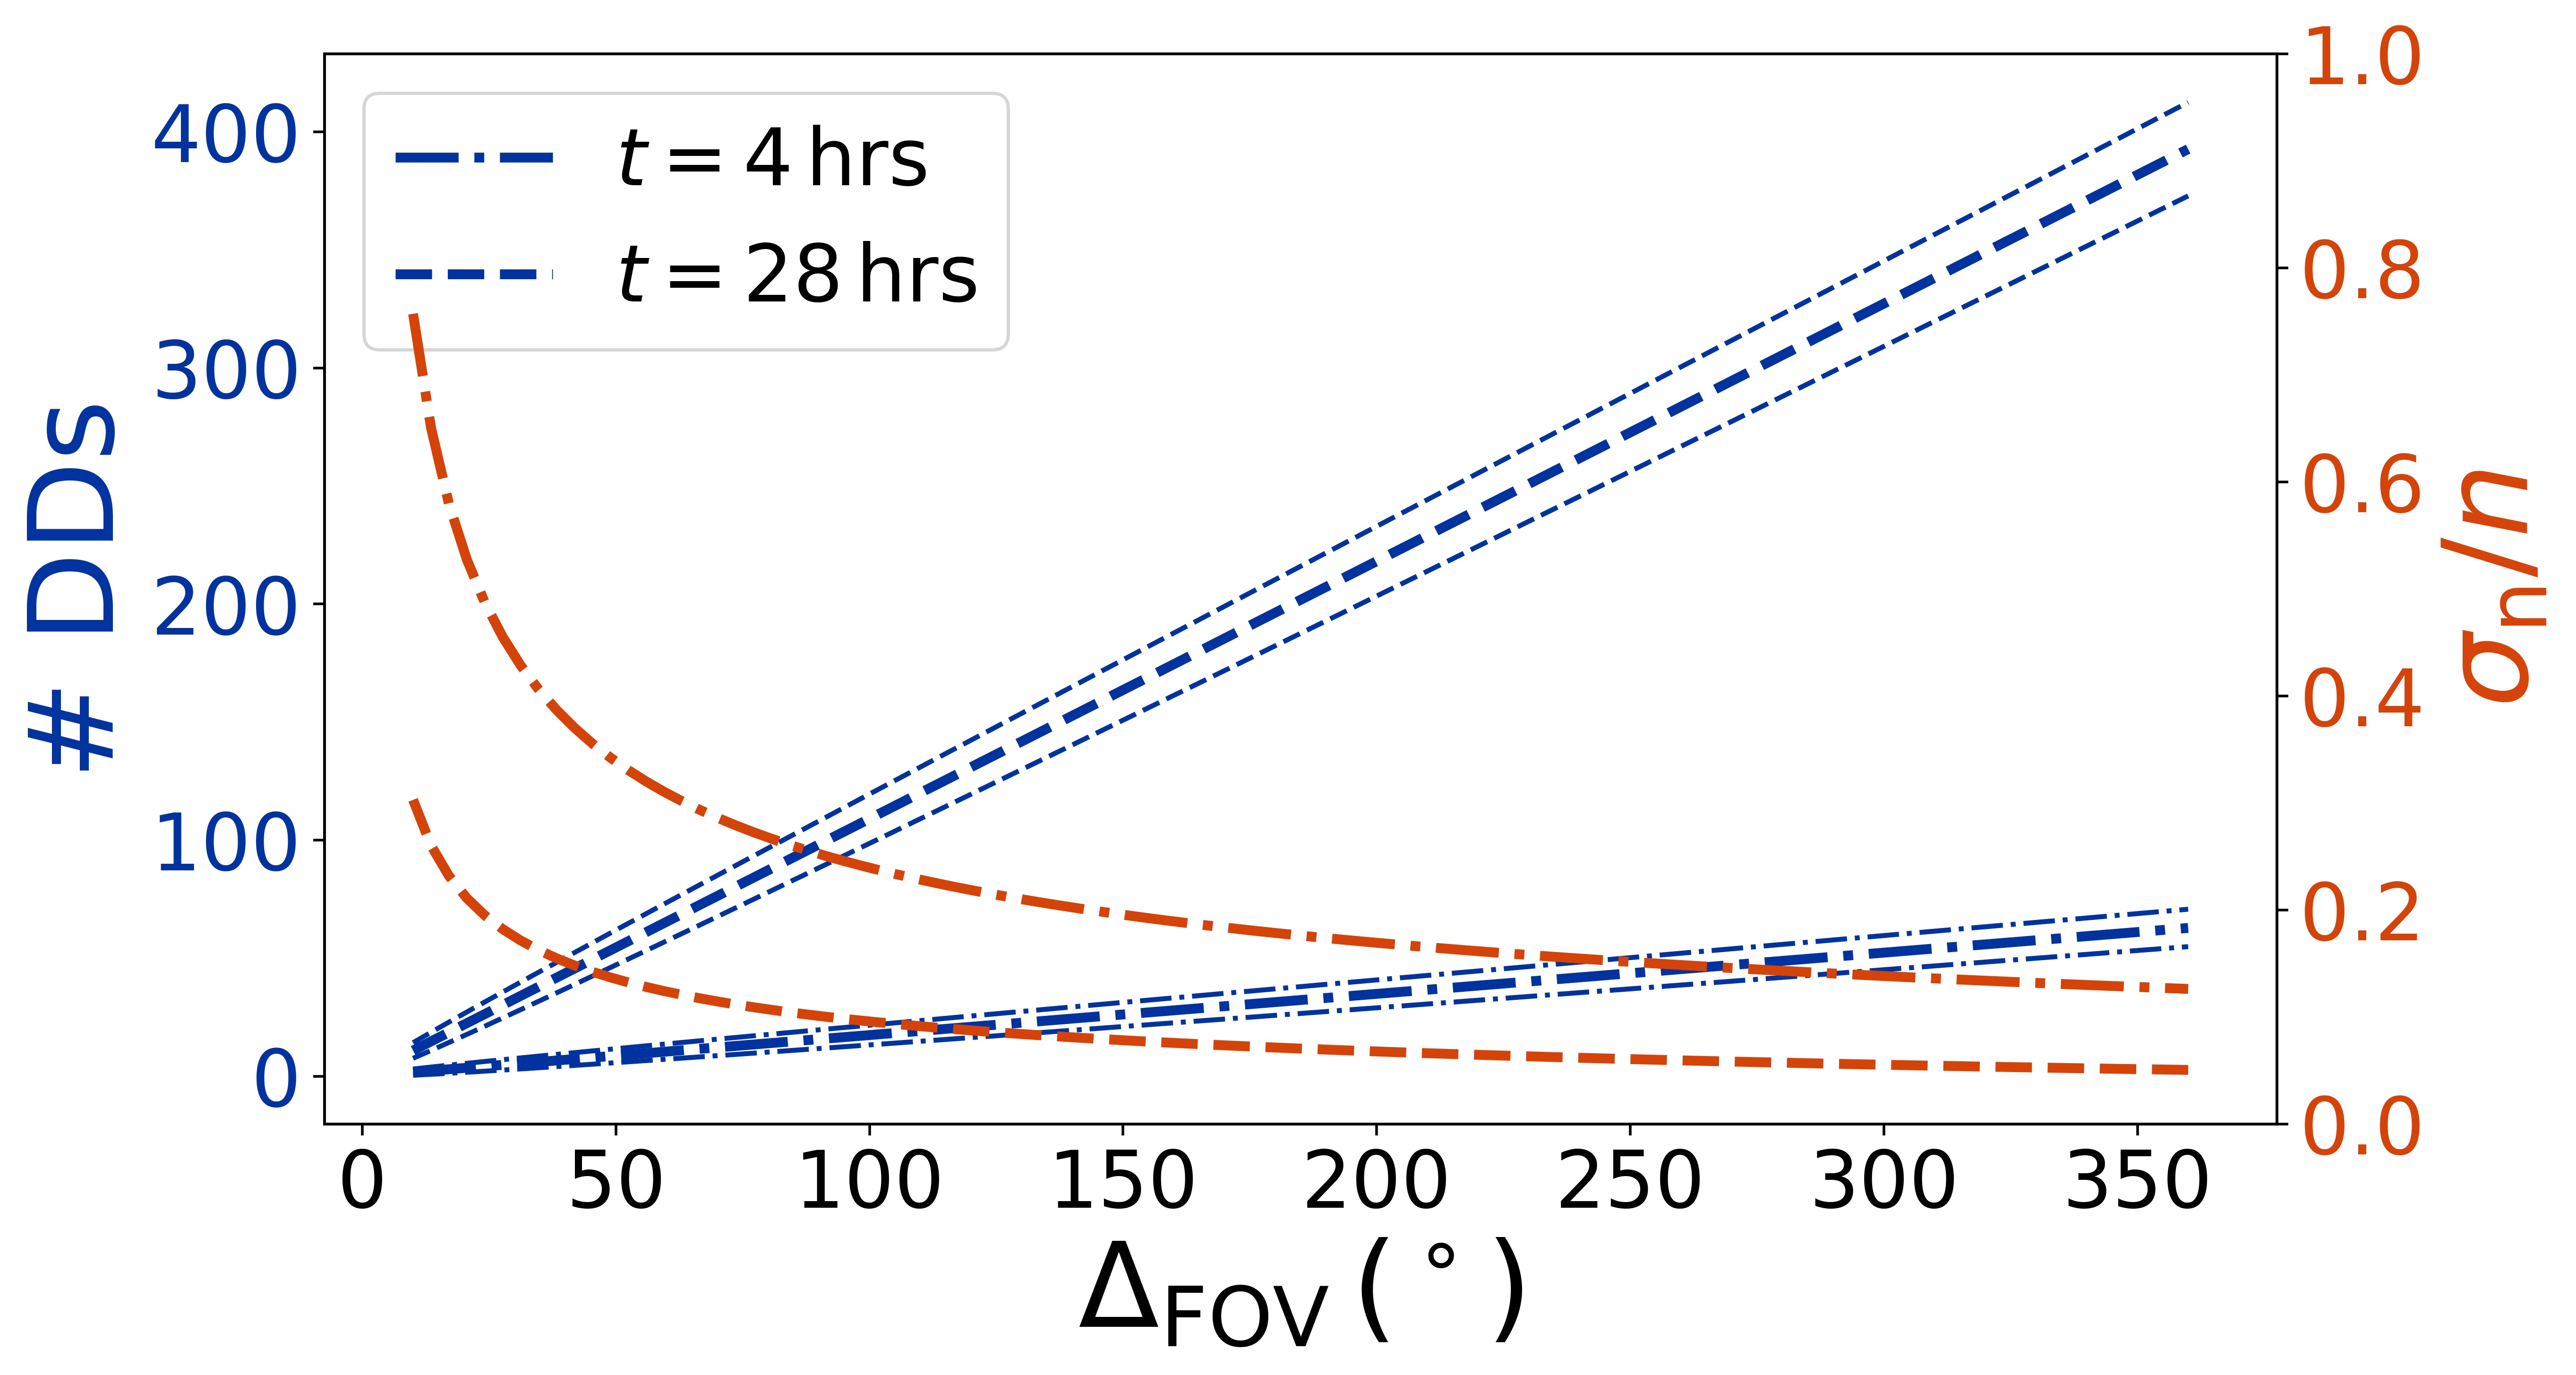
\includegraphics[width=\textwidth]{figures/DDs_vs_Delta.jpg}
    \caption{The number of dust devils recovered by an imaging survey as a function of field-of-view $\Delta_{\rm FOV}$ shown as thick, blue lines, along with estimated uncertainties (adjacent thin, blue lines). The survey precision, $\sigma_n/n$ shown as thick orange lines. The dashed lines of both colors assume a survey duration $t = 4\,{\rm hours}$, and the dash-dot lines a duration $t = 25\,{\rm hours}$.}
    \label{fig:DDs_vs_Delta}
\end{figure}

We can relate the areal occurrence rate $n$ (measured in dust devils per unit area per unit time) from either the areal density of devils $N$ (measured in dust devils per unit area) or the total number of dust devils observed $k$ in an amount of time $t$:
\begin{equation}
   n = \frac{N}{t} = \frac{k}{t A_{\rm survey}} = \left( \frac{2 \alpha^2}{t \Delta_{\rm FOV} D^2} \right)\ k.
    \label{eqn:areal_occurrence_rate}
\end{equation}

If we assume that dust devil occurrence is a Poisson process, then we can estimate the uncertainty on $k$ as $\sigma_k = \sqrt{k}$ and the uncertainty $\sigma_n$ on our estimate of $n$ via
\begin{equation}
    \frac{\sigma_n}{n} = \frac{\sigma_k}{k} = k^{-1/2} = \sqrt{2} \left( n t \right)^{-1/2} D^{-1}\ \Delta_{\rm FOV}^{-1/2} \alpha.
    \label{eqn:sigma_n}
\end{equation}

Usually, we would design our survey so that we achieve a sufficiently precise estimate for the quantity of physical significance $n$. In other words, we would require $\sigma_n/n < T$ with $T$ some threshold. We can see that Equation \ref{eqn:sigma_n} provides the specific requirements to achieve the desired threshold. For instance, we can take some typical values from \citet{2006JGRE..11112S09G} and estimate what minimum angular resolution is required of our camera to achieve $T = 0.1$:
\begin{equation}
    \alpha < 2^{-1/2} T \left( n t \right)^{1/2} D\ \Delta_{\rm FOV}^{1/2} = 2^{-1/2} \left( 0.1 \right) \big[ \left( 0.05\,{\rm km^{-2}\ hr^{-1}} \right) \left( 1\,{\rm hr} \right) \big]^{1/2} \left( 10\,{\rm m} \right) \left( \pi/2\,{\rm rad} \right)^{1/2} \approx 0.2\,{\rm mrad}.
    \label{eqn:alpha_example}
\end{equation}
Such an angular resolution is about ten times better than is usually achieved -- the MER Hazcams used for the survey in \citet{2006JGRE..11112S09G} had a resolution of $2\,{\rm mrad/pix}$ \citep{2003JGRE..108.8071M}.

A more practical application of Equation \ref{eqn:sigma_n} might instead involve assuming values for $\Delta_{\rm FOV}$ and $\alpha$ to estimate the duration required for a survey of a given precision. Taking the same parameters as above but this time with $\alpha \sim 1\,{\rm rad}$, we require a survey of duration $t > 25\,{\rm hr}$ to achieve $T = 0.1$. However, dust devils are usually active only for a few hours during each day (or sol on Mars) -- \citet{2006JGRE..11112S09G} found negligible activity before 9 a.m. LTST or after 5 p.m. LTST. Moreover, the occurrence rate itself seemed to evolve over the course of the active phase, increasing from $0.005\,{\rm km^{-2}\ hr^{-1}}$ early in the morning to  $0.05\,{\rm km^{-2}\ hr^{-1}}$ around noon. This mid-day peak agrees with meteorological predictions that dust devil activity should increase as the planetary boundary layer deepens with increasing surface heating \citep{doi:10.1029/2010RG000351}. Accurately estimating the occurrence rate requires a survey duration not longer than the timescale of variability, i.e., about an hour. Therefore, the 25-hours of survey required to recover $n = 0.05\,{\rm km^{-2}\ hr^{-1}}$ to 10\% accuracy would have to be spread into 1-hour surveys around noon spanning 25 sols. (And, of course, smaller occurrence rates would require additional time.) 

Similarly, \citet{2006JGRE..11112S09G} reported an occurrence rate that varied with season and $L_{\rm S}$. Assuming sufficient daily coverage to accurately capture the daily occurrence rate (i.e., a large enough value for $n t$), we can ask what $\Delta_{\rm FOV}$ might be required to recover the seasonal variability by looking at the expected variation in $n t$. From its peak in spring to the peak in summer, $n t$ dropped from $0.11\,{\rm km^{-2}}$ to $0.05\,{\rm km^{-2}}$, which would require a precision $\sigma_n/n \sim 0.5$. Solving Equation \ref{eqn:sigma_n} gives $\Delta_{\rm FOV} \approx 65^\circ$. Considering instead the maximum $\Delta_{\rm FOV} = 360^\circ$ and an areal occurrence $nt = 0.11\,{\rm km^{-2}}$ suggests we could recover dozens of 10-m wide dust devils. 

Importantly, all these calculations up till now have assumed a single dust devil diameter, $D$. In fact, dust devils span a range of diameters - \citet{2006JGRE..11112S09G} reported values between 2 and $276\,{\rm m}$, while orbital studies have reported devils hundreds of meters across \citep{2008Icar..197...39S}. However, the distribution of diameters appears to follow a steep power law, with an exponent between 1 and 2 \citep{2016SSRv..203..277L}. Consequently, the majority of devils reported in \citet{2006JGRE..11112S09G} lay between 10 and $20\,{\rm m}$, and so $n$ is dominated by devils in this range and the calculations presented so far may be considered reasonably representative. In addition, for a given angular resolution, larger dust devils can be recovered from farther away, an observational bias that has been previously pointed out \citep{2012Icar..219..556K, 2013Icar..226..964L}.

On the other hand, given that larger dust devils are less common, they may be intrinsically less likely to be recovered. Equation \ref{eqn:areal_occurrence_rate} may be adapted to allow for a distribution of dust devils by diameter by simply taking $n$ to represent the areal occurrence rate in a narrow range of diameters and $k$ to represent the number of devils observed within that same range of diameters. From Equation \ref{eqn:areal_occurrence_rate}, we can see that if $n$ were a steeply declining function of $D$ (e.g., $n \propto D^{-3}$), then the total number of devils recovered with smaller diameters would exceed the number with larger diameters in proportion to $D^{-1}$.

Moreover, larger dust devils may dominate the 

\acknowledgments

%% To help institutions obtain information on the effectiveness of their 
%% telescopes the AAS Journals has created a group of keywords for telescope 
%% facilities.
%
%% Following the acknowledgments section, use the following syntax and the
%% \facility{} or \facilities{} macros to list the keywords of facilities used 
%% in the research for the paper.  Each keyword is check against the master 
%% list during copy editing.  Individual instruments can be provided in 
%% parentheses, after the keyword, but they are not verified.

\vspace{5mm}
\facilities{}

%% Similar to \facility{}, there is the optional \software command to allow 
%% authors a place to specify which programs were used during the creation of 
%% the manuscript. Authors should list each code and include either a
%% citation or url to the code inside ()s when available.

\software{}

%% Appendix material should be preceded with a single \appendix command.
%% There should be a \section command for each appendix. Mark appendix
%% subsections with the same markup you use in the main body of the paper.

%% Each Appendix (indicated with \section) will be lettered A, B, C, etc.
%% The equation counter will reset when it encounters the \appendix
%% command and will number appendix equations (A1), (A2), etc. The
%% Figure and Table counter will not reset.

\appendix

% 2020 May 9 - Check notes in notepad from today's date
% \section{Effects of Undersampling the Dust Devil Profile}
% With too low a sampling frequency, the pressure profile for a dust devil will be undersampled, potentially distorting the inferred profile shape and depth. Fourier analysis of the pressure profile can show the dependence of the distortion on the angular sampling frequency $\omega$.

% We start by assuming a Lorentzian profile $L(t)$ in time $t$ for the dust devil:
% \begin{equation}
%     L(t) = -\frac{\Delta P}{1 + \left( t/\Gamma \right)^2},
%     \label{eqn:appendix_lorentzian}
% \end{equation}{}
% where $\Delta P$ is the profile depth and $\Gamma$ its duration. The Fourier transform of this profile $F(\omega)$ is 
% \begin{equation}
%     F(\omega) = -\pi \Delta P\ \Gamma e^{-|\omega| \Gamma}.
%     \label{eqn:appendix_lorentzian_fourier}
% \end{equation}{}

% If we now imagine that we undersampled the profile using frequencies below some maximum, $\omega \le \omega_{\rm max}$, then we can estimate the resulting distorted profile $L^\prime(t)$ by taking the inverse, partial Fourier transform of $F(t)$, i.e.
% \begin{equation}
%     L^\prime(t) \equiv \int_{\omega = -\omega_{\rm max}}^{\omega_{\rm max}}\ \left( -\pi \Delta P \Gamma e^{-|\omega| \Gamma}\right) \ \left( \frac{e^{+i\omega t}\ d\omega}{2 \pi} \right)
%     = L(t) \bigg[ 1 - \left( \cos \left( \omega_{\rm max} t \right) - \left( \frac{t}{\Gamma} \right) \sin \left( \omega_{\rm max} t \right) \right) e^{-\omega_{\rm max} \Gamma} \bigg].
%     \label{eqn:appendix_inverse_fourier}
% \end{equation}{}

% We expect the register the maximum (in magnitude) pressure excursion at the center of the profile, i.e. $L(t = 0) = \Delta P$, and so to estimate the incorrect profile depth $\Delta P^\prime$ arising from this distorted profile, we can evaluate $L^\prime(t)$ at the same time, giving:
% \begin{equation}
%     \Delta P^\prime = \Delta P \left( 1 - e^{-\omega_{\rm max}\Gamma} \right).
% \end{equation}{}
% The distortion decreases rapidly with $\omega_{\rm max}$, and for a sampling frequency of, for example, $2\,{\rm Hz}$ ($\omega_{\rm max} = 2\pi \times (2\,{\rm Hz})$) and a very narrow profile $\Gamma = 0.5\,{\rm s}$, $\Delta P^\prime$ is only 0.2\% different from $\Delta P$.

\bibliography{sample63}{}
\bibliographystyle{aasjournal}

%% This command is needed to show the entire author+affiliation list when
%% the collaboration and author truncation commands are used.  It has to
%% go at the end of the manuscript.
%\allauthors

%% Include this line if you are using the \added, \replaced, \deleted
%% commands to see a summary list of all changes at the end of the article.
%\listofchanges

\end{document}

% End of file `sample63.tex'.
